\chapter{Concept}\label{Chap:Concept}

For further reading the to be built system will be called "Parametrised Augmented Reality Robot Human Interface" (\textit{PARRHI}).

\section{Goal}
As described in section \ref{Section:PARRHIApproach} this thesis presents a possible approach to solve the previously described problems (see section \ref{Section:ProblemDescription}). It is the main target of this bachelor's thesis to remove the necessity of high software engineering skills to develop reasonably complex Augmented Reality Robot Human Interface applications, maintaining the quality of the outcome and even increasing the degree of resuability. This might result in lower development costs, lower struggle to gather software engineering talent and even in a shorter time to market.

To succeed in this goal, a specific set of requirements has to be defined and documented in a formal way. To gather these requirements the V-Model developed by the Federal Republic of Germany was used~\cite{vmodell}.

\section{User Requirements}
Before defining the User Requirements the system's end user has to be defined. The characteristics of the actual enduser of \textit{PARRHI} might be someone who:
\begin{itemize}
	\setlength\itemsep{-1em}
	\item Knows the basics of text editing software,
	\item has no qualifications in software engineering,
	\item wants to develop an Augmented Reality application for professionals that collaborate with industrial robots in a shared perimeter.
\end{itemize}

Having an idea of the end-user, the user-requirements can be defined. The user wants to:
\begin{itemize}
	\setlength\itemsep{-1em}
	\item Develop a AR-applications without software engineering skills
	\item Have the tools necessary to create medium complex applications for use cases such as tutorials, maintenance instructions or other teaching purposes
	\item Build upon other people's work or projects
	\item Launch the AR-application on a suitable device
	\item Possibly use the same system on different types and brands of robots
\end{itemize}

\section{System Requirements}\label{Section:SystemRequirements}
Deriving from the previous chapter the System should:
\begin{enumerate}
	\setlength\itemsep{-1em}
	\item have input data in a non-code format.
	\item have readable and intuitive feedback on the input data.
	\item achieve reusablity by having an input in non-binary text format that allows copy and paste reproduction.
	\item support building for hand held mobile devices and head mounted Augmented Reality glasses.
	\item allow bidirectional communication (Sending commands and receiving data) with the robot's controller 
	\item allow documentation of the applications workflow
	\item be as platform independent as possible
\end{enumerate}

\section{PARRHI Concept}
\begin{figure}
	\centering
	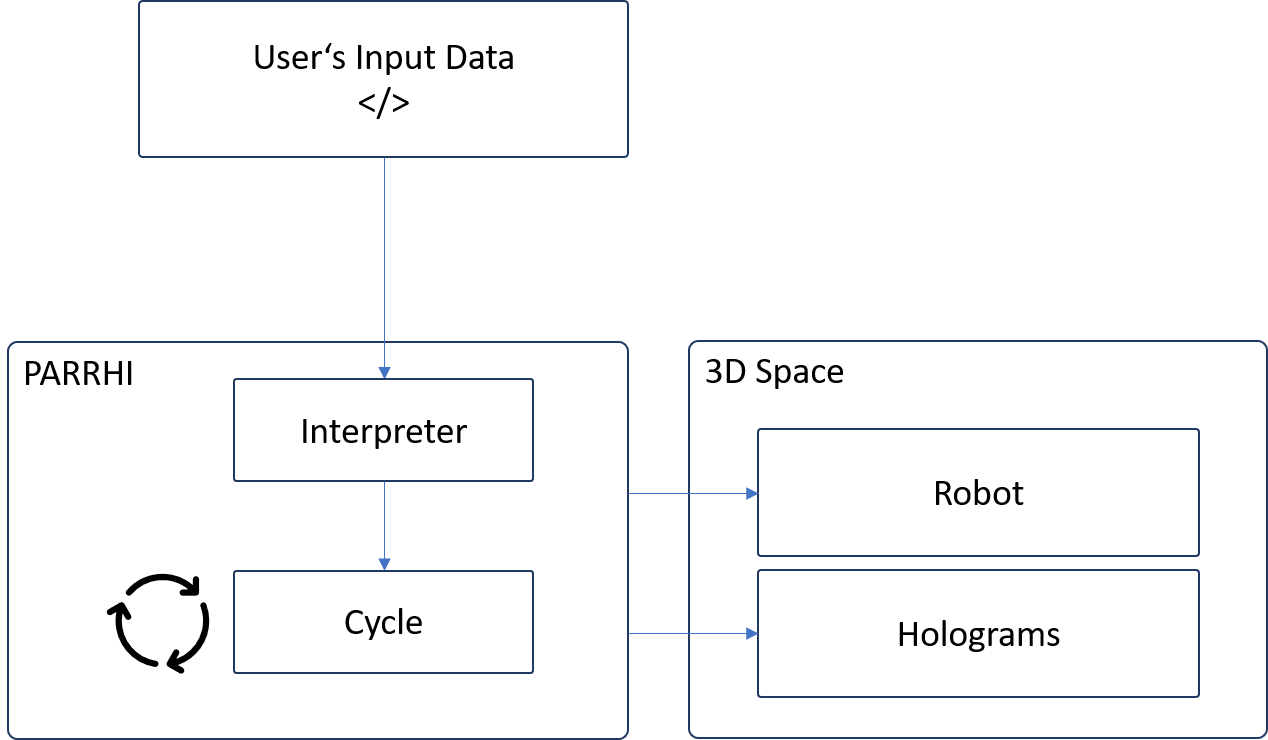
\includegraphics[width=0.75\textwidth]{Figures/PARRHIConcept01.png}
	\caption{PARRHI general concept}
	\label{Fig:PARRHIConcept}
\end{figure}


\textit{PARRHI} basically consists of three components (see Fig. ~\ref{Fig:PARRHIConcept}):
\begin{enumerate}
	\setlength\itemsep{-1em}
	\item Input Data
	\item PARRHI Engine
	\item the "real world"
\end{enumerate}

\textit{Input Data} file, which is created by the application's developer, represents \textit{PARRHI's} only input. It contains a set of definitions, commands and behaviour rules that are necessary to create AR Interfaces that is able to fulfil the defined requirements in \ref{Section:SystemRequirements}.

The \textit{PARRHI Engine} interprets the input data and acts on its behalf. After validating the input data against certain schemes the engine imports all contents and sets up its internal states, before entering a cyclic mode - ready for operation.

\subsection{Input Data}

The Input Data is hierarchically structured in four main parts, each containing different sub-elements to further specify their function. 

\begin{table}
	\caption{\textit{Input Data} structure}
	\label{Tab:InputDataStructure}
	\centering
	\begin{tabular}{lcl}
		\toprule
		Name & Section		& Explanation	\\		
		\midrule
		Variables & \ref{Section:Variables}		& Integer variables to create state machines \\
		Points& \ref{Section:Points}		& \parbox[t]{10cm}{Different kinds of 3D Point definitions\\(fix, relative to the robot, relative to the user)} 	 \\
		Holograms& \ref{Section:Holograms} & Holograms can be mounted onto points and have a set of properties\\
		Events& \ref{Section:Events} & Events have certain triggers and carry two Actions as a payload \\
		\bottomrule
	\end{tabular}
\end{table}

\subsubsection{Variables}\label{Section:Variables}
\textit{PARRHI's} variables can be used to create different steps in one's application. Variables can be the source of an event's trigger or the target of an event's action. To see how events work, see \ref{Section:Events}.

\subsubsection{Points}\label{Section:Points}
Points are a three dimensional vectors that can be defined in three different ways. There is a \textit{Fix-Point} that has static coordinates. It could be used to setup holograms that visualize certain spacial environmental constraints or for different steps in a \textit{PARRHI} AR-HR-Interface application. 


\tdplotsetmaincoords{60}{120} 
\begin{tikzpicture} [scale=0.01, tdplot_main_coords, axis/.style={->, black, thick}, 
vector/.style={-stealth,black,thick}, 
vector guide/.style={dashed,gray,thin}]

%standard tikz coordinate definition using x, y, z coords
\coordinate (O) at (0,0,0);

%tikz-3dplot coordinate definition using x, y, z coords

\pgfmathsetmacro{\ax}{100}
\pgfmathsetmacro{\ay}{100}
\pgfmathsetmacro{\az}{200}
\pgfmathsetmacro{\axSize}{200}

\coordinate (P) at (\ax,\ay,\az);

%draw axes
\draw[axis] (0,0,0) -- (\axSize,0,0) node[anchor=north east]{$x$};
\draw[axis] (0,0,0) -- (0,\axSize,0) node[anchor=north west]{$y$};
\draw[axis] (0,0,0) -- (0,0,\axSize) node[anchor=south]{$z$};

%draw a vector from O to P
\draw[vector] (O) -- (P);

%draw guide lines to components
\draw[vector guide]         (O) -- (\ax,\ay,0);
\draw[vector guide] (\ax,\ay,0) -- (P);
\draw[vector guide]         (P) -- (0,0,\az);
\draw[vector guide] (\ax,\ay,0) -- (0,\ay,0);
\draw[vector guide] (\ax,\ay,0) -- (0,\ay,0);
\draw[vector guide] (\ax,\ay,0) -- (\ax,0,0);
\node[tdplot_main_coords,anchor=north]
at (\ax+100,0,-60){(\ax, 0, 0)};
\node[tdplot_main_coords,anchor=west]
at (0,\ay,50){(0, \ay, 0)};
\node[tdplot_main_coords,anchor=south]
at (0,0,\az+50){(0, 0, \az)};
\end{tikzpicture}

To interact with the robot \textit{PARRHI} needs a way to read and display data from the robot. For that, there are \textit{Robot-Points} that are defined by the index of two joints and a scalar value that defines the exact location (linear interpolation) between them.

\tdplotsetmaincoords{60}{120} 
\begin{tikzpicture}  [scale=0.03, tdplot_main_coords, axis/.style={->, black, thin}, 
vector/.style={-stealth,green,very thick}, 
robot/.style={green, very thick},
vector guide/.style={dashed,gray,thin}]

%standard tikz coordinate definition using x, y, z coords
\coordinate (O) at (0,0,0);

%tikz-3dplot coordinate definition using x, y, z coords


\pgfmathsetmacro{\axSize}{100}
\pgfmathsetmacro{\jointRadius}{50}

%Robot Points in cm (mm too large dimensions for library)
\coordinate (P0) at (0,0,0);
\coordinate (P1) at (5,0,33);
\coordinate (P2) at (5, 0, 77);
\coordinate (P3) at (15, 0, 100.5);
\coordinate (P4) at (47, 0, 100.5);
\coordinate (P5) at (55, 0, 100.5);
\coordinate (P6) at (63, 0, 100.5);
\coordinate (Point) at (5, 0 , 60);


%draw coordinate system axes
\draw[axis] (0,0,0) -- (\axSize,0,0) node[anchor=north east]{$x$};
\draw[axis] (0,0,0) -- (0,\axSize,0) node[anchor=north west]{$y$};
\draw[axis] (0,0,0) -- (0,0,\axSize) node[anchor=south]{$z$};

%draw the robot's joints and axes
\draw[robot] (P0) -- (P1); \fill[fill=gray] (P0) circle (\jointRadius pt);
\draw[robot] (P1) -- (P2); \fill[fill=gray] (P1) circle (\jointRadius pt);
\draw[robot] (P2) -- (P3); \fill[fill=gray] (P2) circle (\jointRadius pt);
\draw[robot] (P3) -- (P4); \fill[fill=gray] (P3) circle (\jointRadius pt);
\draw[robot] (P4) -- (P5); \fill[fill=gray] (P4) circle (\jointRadius pt);
\draw[robot] (P5) -- (P6); \fill[fill=gray] (P5) circle (\jointRadius pt);

%Draw PointRowot
\fill[fill=black] (Point) circle (\jointRadius pt);

%draw the 
\node[tdplot_main_coords,anchor=east]
at (P1){(Joint 1)};
\node[tdplot_main_coords,anchor=west]
at (P2){(Joint 2)};
\node[tdplot_main_coords,anchor=west]
at (Point){(Point scalar = 0.6)};




\end{tikzpicture}

\subsubsection{Holograms}\label{Section:Holograms}
\subsubsection{Events}\label{Section:Events}














